\chapter{Diskussion}
\label{kap:diskussion}

Die Auswertungen der experimentellen Daten durch einen Biexponentiellen Zerfall lieferte robuste Parameterschätzungen (für $k_1$, $k_2$ und $A$), wenn ausreichend Datenpunkte für den schnellen und langsamen Prozess vorhanden waren und $A \approx 0,5$. Robust bedeutet, dass die Fehler der Fitparameter mindestens eine Größenordnung kleiner sind als der Wert des Fitparameters selbst. In den Force-Clamp-Experimenten bei den pH-Werten 8, 7,4 und 4,5 erfüllte ausschließlich das Force-Clamp-Experiment bei pH 7,4 diese Kriterien. Bei pH 8 fielen nur 5 Datenpunkte in den schnellen Prozess, sodass $\Delta k_1^{8}  \approx k_1^{8}$. Bei pH 4,5 war nicht mit Sicherheit zu sagen ob ein schneller Prozess vorhanden war, da nur 2 Datenpunkte in diesen Prozess vielen.\\
Interessant ist jedoch generell das Auftreten eines schnellen und eines langsamen Prozesses. Es stellen sich daher die Fragen:

\begin{itemize}
	\item Welcher Prozess stellt die Hydrolyse der \amid~ dar?
	\item Was bedeutet der andere Prozess?
\end{itemize}

Um zu zeigen, dass die \amid~ in der Kette zwischen Substrat, \spacer~ und \spitze~ das schwächste Glied war, wurden in einer anderer Arbeit folgende Kontrollen durchgeführt~\cite{ClausenSchaumann.2018}:

\begin{itemize}
	\item Austausch der \aminos~auf Substrat und \spitze~durch \carboxys~(Bildung von Esterbindungen zwischen \ac{CMA} und Substrat/ \spitze)
	\item Austausch von \ac{CMA} durch Biscarboxy-PEG bzw. Adipinsäure (keine glykosidischen Bindungen innerhalb des \spacers)
\end{itemize}

%%% Fußnotentext
\renewcommand{\noteOne}{Die Dissoziationsenergie der O-O-Bindung liegt bei $142~kJ~mol^{-1}$. Verglichen mit einer C-C-Bindung mit $339~kJ~mol^{-1}$ oder C-O-Bindung mit $331~kJ~mol^{-1}$ um mehr als die Hälfte schwächer \cite[15]{Latscha.2016}}
%%% Endefußnotentext


Wurde in einem Force-Clamp-Experiment an einer Esterbindung gemessen, lag $\tau$ bei ca. 4 Sekunden. Wurde der \spacer~durch Biscarboxy-PEG oder Adipinsäure ersetzt und an der Amidbindung gemessen lag $\tau$ bei ca. 0,17 Sekunden. All diese Experimente wurden bei pH = 7,4 durchgeführt. Ein Vergleich von \cite{ClausenSchaumann.2018} und den hier durchgeführten Force-Clamp-Experimenten lässt vermuten, dass es sich bei dem schnellen Prozess um die Hydrolyse der \amid~handelte. Demnach konnte es sich bei dem langsamen Prozess nicht um die Beeinflussung der \amid~durch den Einbau von \ch{O2} während der Funktionalisierung des Substrats/ \spitze~handeln (s. Abschnitt~\ref{subsec:oberflächenfunktionalisierung_via_kohlenstoffanker}). Wird davon ausgegangen, dass sich Peroxidbrücken gebildet hätten, wäre die Wahrscheinlichkeit hoch, dass diese während der Oberflächenfunktionalisierung unter UV-Lichteinwirkung (λ= 254 nm) homolytisch gespalten worden wären\footnote{\noteOne}. Prinzipiell wären dann folgende Reaktionen möglich: 


\begin{eqnarray}
	\ch[arrow-min-length=2cm]{S-O-O-R1	&	->[$h\nu$]	&	S-O. + .O-R1} \label{scheme:peroxid_step_1}\\
	\ch[arrow-min-length=2cm]{S-O. + R2 + H.	&	->	&	S-O-R2H} \label{scheme:peroxid_step_2}\\
	\ch[arrow-min-length=2cm]{S-O. + H.	&	->	&	S-OH} \label{scheme:peroxid_step_3}\\
	\ch[arrow-min-length=2cm]{R3 + .O-R1 + H.	&	->	&	HR3-O-R1} \label{scheme:peroxid_step_4}\\
	\ch[arrow-min-length=2cm]{H. + .O-R1	&	->	&	HO-R1} \label{scheme:peroxid_step_5}
\end{eqnarray}

Wobei $R_1$, $R_2$ und $R_3$ jeweils für unterschiedliche Allylamin-Moleküle und $S$ für das Substrat (wahlweise auch für die \spitze) stehen. Hier wurde das baumartige Wachstum von Allylamin auf dem Substrat bzw. der Abtastspitze nicht berücksichtigt. Unter der Annahme, dass sich die Peroxidbrücken (Reaktion~\ref{scheme:peroxid_step_1}) gespalten hätten, wäre die Wahrscheinlichkeit dafür, dass die Peroxide im Laufe der Funktionalisierung zu Ethern reagierten (Reaktion~\ref{scheme:peroxid_step_2}) sehr hoch (vgl.~\cite[15]{Latscha.2016}). Die Reaktionen~\ref{scheme:peroxid_step_3}~bis~\ref{scheme:peroxid_step_5} würden die Ausbeute der Funktionalisierung herabgesetzten und die Ausbildung einer \amid~verhindern. Die Etherbrücken, gebildet nach Reaktion~\ref{scheme:peroxid_step_2}, waren unter Krafteinfluss jedoch stabiler als die \amid~(vgl.~\cite{ClausenSchaumann.2018}) und wären damit nicht in den durchgeführten Force-Clamp-Experimenten sichtbar gewesen. Dabei wird davon ausgegangen, dass sich der Sauerstoff zwischen Substrat und der \amid~befindet und somit an Ether und an Amid gleichzeitig gemessen wurde. Auch die Bildung von Estern, statt der Amide, durch die Einführung von Hydroxylgruppen auf dem Substrat bzw. der \spitze~wie in Reaktion~\ref{scheme:peroxid_step_3} gezeigt ist, wäre möglich, jedoch entspricht keine der hier ermittelten mittleren Lebensdauern der langsamen Prozesse der des Esters ($\tau_{Ester}  = 4~s$) aus \cite{ClausenSchaumann.2018}.\\

Weitere Ursachen, die den langsamen Prozess hervorrufen:

\begin{itemize}
	\item Das Auftreten einer zweiten Bindungsart
	\item Beeinflussung der Amidhydrolyse
	\item Mehrfach, parallel gebildete \amide~zwischen den \carboxys~eines einzigen \spacer~an Substrat und \spitze
\end{itemize}

%% Fußnotentext
\renewcommand{\noteOne}{Abgesehen von Hydroxylgruppen. Die daraus resultierenden Ester konnten anhand ihrer mittleren Lebensdauer für den langsamen Prozess ausgeschlossen werden (s.o.).}

\renewcommand{\noteTwo}{Die nukleophile Addition von \ch{H2O} an das Carbonylkohlenstoff ist die initiale Reaktion für die Hydrolyse. Diese Reaktion kann durch Säuren oder Basen beschleunigt werden 	\cite[288]{Latscha.2016}}

\renewcommand{\noteThree}{Die Reaktivität der Carbonsäurederivate beruht auf der Basizität des Substituenten. Je geringer die Basizität, desto stabiler ist das Derivat. Die Einteilung nach steigender Reaktivität lautet dabei wie folgt \cite[287]{Latscha.2016}:
	\scalebox{0.9}{
		\setchemfig{scheme debug = false}
		\setchemfig{angle increment=30}
		\definesubmol{rest}{R-[,0.75]C(=[2,0.75]O)-[-2,0.75]}
		\schemestart
		\chemname{
			\chemfig{!{rest}OH}
		}{Carbonsäure}
		\arrow(.base east--.base west){0}[,0]<\arrow(.base east--.base west){0}[,0.3]
		\chemname{
			\chemfig{!{rest}NH_2}
		}{-amid}
		\arrow(.base east--.base west){0}[,0]<\arrow(.base east--.base west){0}[,0.3]
		\chemname{
			\chemfig{!{rest}OR}
		}{-ester}
		\arrow(.base east--.base west){0}[,0]<\arrow(.base east--.base west){0}[,0.3]
		\chemname{
			\chemfig{!{rest}SR}
		}{-thioester}
		\arrow(.base east--.base west){0}[,0]<\arrow(.base east--.base west){0}[,0.3]
		\chemname{
			\chemfig{R-[,0.75]C(=[2,0.75]O)-[-1,0.75]O-[1,0.75]C(=[4,0.75]O)-[,0.75]R}
		}{-anhydrid}
		\arrow(.base east--.base west){0}[,0.3]<\arrow(.base east--.base west){0}[,0.3]
		\chemname{
			\chemfig{!{rest}Cl}
		}{-chlorid}
		\schemestop
	}
}
%%% Ende Fußnotentext

Der langsame Prozess könnte über eine zweite Bindungsart erklärt werden, wenn angenommen wird, dass die Oberflächen von Substrat und \spitzen~mit anderen funktionellen Gruppen ausgestattet worden wären\footnote{\noteOne}, oder ein Tausch der funktionellen Gruppen stattgefunden hätte. Für beides wären jedoch spezielle Substanzen nötig, die nicht zufällig durch unsauberes Arbeiten eingebracht werden konnten. Das Auftreten einer zweiten Bindungsart kann daher ausgeschlossen werden.\\

Es bleibt bisher ungeklärt, welche Reaktionen generell an sekundären Carbonsäureamiden ablaufen können. Die Frage ist wie sich etwaige Verunreinigungen oder Reaktionsnebenprodukte auf die \amid~auswirkten. Die typische Angriffspunkte der Carbonsäureamide sind die Carbonylgruppe (\abb~\ref{fig:amidbindung}, Position~1) und das C-Atom in $\alpha$-Stellung zur Carbonylgruppe (\abb~\ref{fig:amidbindung}, Position~2). An diesen Stellen wären eine Reihe von Reaktionen möglich \cite[305-308]{Latscha.2016}. An der Carbonylgruppe könnten in erster Linie Additionsreaktionen (sowohl nukleophil\footnote{\noteTwo} durch den Angriff am Carbonylkohlenstoff oder elektrophil durch den Angriff an der Doppelbindung der Carbonylgruppe) durchgeführt werden. Daneben könnte die Carbonylgruppe reduziert, bzw. oxidiert werden. Das Kohlenstoffatom in $\alpha$-Stellung könnte deprotoniert werden und so das Carbonsäureamid in seine Enolatform überführt werden. An der entstandenen Doppelbindung zum $\alpha$-C-Atom können wiederum elektrophile Additionsreaktionen durchgeführt werden. Da Carbonsäureamide zu den schwach reaktiven Carbonsäurederivaten\footnote{\noteThree} zählt, sind für die oben genannten Reaktionen jedoch starke Reagenzien notwendig. Reaktionen am Stickstoffatom finden nicht statt. Zum einen war die Basizität durch eine Keto-Enol-Tautomerie der C-N-Bindung und zum anderen die N-H-Acidität durch +I-Effekte der Substituenten am Stickstoffatom herabgesetzt. 

% Reaktionspositionen der Amidbindung
\begin{figure}[h]
	\centering
	\scalebox{0.5}{
		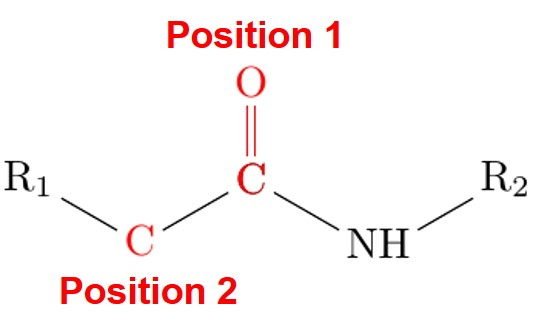
\includegraphics[width=\linewidth]{Abbildungen/amide_bond_II.jpg}
	} % scalebox
	\caption[Amidbindung eines Carbonsäureamids]{Amidbindung eines Carbonsäureamids. Position~1: Carbonylgruppe. Position~2: C-Atom in $\alpha$-Stellung zur Carbonylgruppe. $R_1$ steht für den Allylaminrest an Substrat/ \spitze, $R_2$ für die Fortsetzung des \acs*{CMA}-Spacers.}
	\label{fig:amidbindung}
\end{figure}

Eventuelle Verunreinigungen oder Reaktionsnebenprodukte der einzelnen Funktionalisierungen können sich entweder auf die Kinetik, oder den Mechanismus der Amidhydrolyse auswirken. Die Kinetik ändert sich, wenn die Aktivierungsenergien der \ac{UZ} geändert werden, oder der Übergang von \ac{TZP} zu \ac{ZI} erleichtert bzw. behindert wird.\\
Für eine Änderung des Reaktionsmechanismus muss die Struktur der Amidbindung durch chemische Reaktionen geändert werden.\\

Die Beeinflussung der Hydrolyse durch Reaktionsnebenprodukte kann jedoch ausgeschlossen werden, da sie durch die jeweiligen Waschschritte entfernt worden sind. Quellen für sonstige Verunreinigungen sind vor allem organische Rückstände (hauptsächlich Fette) oder Mineralablagerungen (\ch{CaCO3} und \ch{MgCO3}) auf den Oberflächen der verwendeten Petrischalen und Pinzetten. Da organische Ablagerungen in Form von Fetten unlöslich sind, würden sie als Oberflächenfilm auf die Substrate übertragen und die Bildung von \amide~an diesen Stellen verhindern. Mineralablagerungen sind in wässrigen Medien schwer löslich und kommen in äußerst geringen Mengen vor (maximal $1~mg$). Verglichen mit dem Volumen der \ac{PBS}-Lösungen in den verwendeten Petrischalen (ca. $5~ml$) wäre die Konzentration von \ch{CaCO3} bzw. \ch{MgCO3} mit $c \approx 2~mmol~l^{-1}$ sehr nahe bei null. Mögliche Änderungen des pH-Wertes, sowie ionische Einflüsse von \ch{Ca^2+}- bzw. \ch{Mg^2+}-Ionen sind damit Vernachlässigbar.\\
Eventuelle ionische Effekte auf die Kinetik der Amidhydrolyse würden sich auf alle Experimente (hier durchgeführte Force-Clamp-Experimente, sowie die Kontrollen in \cite{ClausenSchaumann.2018}) gleichermaßen auswirken und die Hydrolysereaktion entweder beschleunigen, oder verlangsamen, jedoch nicht beides zur gleichen Zeit.\\

Um die Struktur der Amidbindung zu ändern, sind zwei Reaktionen von Bedeutung~\cite[301\psqq]{Latscha.2016}: 

\begin{itemize}
	\item Reduktion der Carbonylgruppe (Position 1, \abb~\ref{fig:amidbindung})
	\item Deprotonierung des $\alpha$-C-Atoms (Position 2, \abb~\ref{fig:amidbindung})
\end{itemize} 

Für die Reduktion der Carbonylgruppe sind jedoch starke Reduktionsmittel wie \ch{LiAlH4} notwendig \cites[306]{Latscha.2016}[208]{Leisering.2017}. Es ist sehr unwahrscheinlich, dass solche Verbindungen als Verunreinigung von außen eingetragen wurden. Die Deprotonierung des $\alpha$-C-Atoms bedarf starker Basen und verläuft sehr langsam~\cites[308]{Latscha.2016}[122]{Hadener.2006}. Die pH-Werte der Force-Clamp-Experimente lagen jedoch zwischen 4,5 und 8, waren für diese Reaktion daher zu niedrig. Daneben verläuft diese Reaktion viel langsamer als die Amidhydrolyse unter Krafteinfluss. Vor diesem Hintergrund können Verunreinigungen, sowie Reaktionsnebenprodukte als Grund für den langsamen Prozess ausgeschlossen werden.\\

Eine plausiblere Erklärung für den langsameren Prozess sind Mehrfachanbindungen des \spacer~an Substrat und \spitze, wie in \abb~\ref{fig:multiple_bonding} dargestellt ist \cite{Grandbois.1999}. 

\begin{figure}[H]
	\centering
	\scalebox{0.3}{
		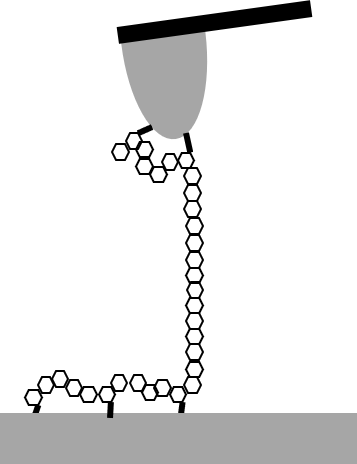
\includegraphics[width=\linewidth]{Abbildungen/Mehrfachanbindung_II.png}
	} % scalebox
	\caption[Mehrfachanbindungen]{Mehrfach angebundener \acs*{CMA}-Spacer an Substrat und \spitze.}
	\label{fig:multiple_bonding}
\end{figure}

%% Fußnotentext
\renewcommand{\noteOne}{Das Zufällig mehrere \spacer~gleichzeitig gestreckt und somit an mehreren Amidbindungen parallel gemessen wurde, kann ausgeschlossen werden. Zum einen zeigten die Kraft-Abstands-Kurven das typische Plateau von \ac{CMA} in einem Bereich von $300$ bis $400~pN$, zum aneeren zeigt die Überlagerung mehrerer Normierter Kraft-Abstands-Kurven dieser Clampereignisse keine Abweichung der mechanischen Polymereigenschaften.}


%% Ende Fußnotentext

Um im Falle eines einzelnen \ac{CMA}-Moleküls, dass über mehrere \amid~an Substrat und \spitze~gekoppelt wurde, Einzelabrisse in den Kraftkurven identifizieren zu können,  (s. Abschnitt~\ref{subsec:auflösungsgrenzen_der_kraftexperimente}) müssen die Abstände der Anbindungen groß genug sein (s.u.). Sind die Abstände zu klein überlagern sich die Einzelereignisse und abhängig von der Anzahl der vorhandenen \amide~errechnet sich so eine Geschwindigkeitskonstante, die erheblich größer ist, als sie für eine einzelne Bindung zu erwarten wäre. Wie in Abschnitt~\ref{subsec:auflösungsgrenzen_der_kraftexperimente} gezeigt wurde, liegt die Auflösungsgrenze in z-Richtung bei $\Delta l_{min} = 1~nm$. Die Monomerlänge von Amylose beträgt $l_{mono} = 0,36~nm$. Rechnerisch müssten die Amidbindungen daher mindestens 3 Monomereinheiten auseinander liegen um noch als Einzelabriss erkannt zu werden. In der Regel wurde dieser Wert durch das thermische Rauschen erhöht. Die Amplitude des thermischen Rauschens betrug im mittel ca. $40~pN$ was für typische Federkonstanten von $0,08~N~m^{-1}$ einen Wert von ca. $1~nm$ entspricht. Damit Mehrfachabrisse klar als diese erkannt werden können, sollten sie daher die doppelte Länge, also ca. $2~nm$ (6 Monomereinheiten) lang sein. Das während eines Clamp-Experiments unerkannte Mehrfachabrisse auftraten, ist hinsichtlich der langen Reaktionszeit an der Oberfläche durchaus möglich (die Wartezeit im 2. Segment betrug $3~s$). Das Zufällig mehrere \spacer~gleichzeitig gestreckt und somit mehrere Amidbindungen parallel gemessen wurden, kann ausgeschlossen werden. Zum einen zeigten die Kraft-Abstands-Kurven das typische Plateau von \ac{CMA} bei $300$ bis $400~pN$, zum anderen zeigt die Überlagerung mehrerer normierter Kraft-Abstands-Kurven dieser Clampereignisse keinen Unterschied in den mechanischen Eigenschaften (s. Anhang~\ref{appendix:A}). Die quantitative Bestimmung der mechanischen Eigenschaften nach dem Modell der frei verbundenen Kette unterstützt diese Aussage (s. Anhang~\ref{appendix:B}).\\
 Ein weiterer Effekt, der die Amidhydrolyse beeinflusste, war der thermische Drift. Dieser schwankte zwischen $1~pN~s^{-1}$ und $5~pN~s^{-1}$. Die Zeit, bis die Amidbindung auf ca. $800~pN$ gestreckt wurde betrug ca. $4~s$. Die eingestellte Kraft schwankte dadurch zwischen $600$ und $800~pN$. Beides zusammen, das Messen von Mehrfachanbindungen und eine stark schwankende Clamp-Kraft, führte bei einigen Force-Clamp-Experimenten zu einer Überschätzung der Amidbindung, wodurch die lange mittlere Lebensdauer ($\tau \approx 20~s$) des langsamen Prozesses erklärt werden kann.\\

Der schnelle Prozess mit $k_1$ stellt die Hydrolyse zur Amidbindung dar. Im basischen Bereich (pH = 8) ist $k_1^8~=~5,3~s^{-1}$ und somit größer im Vergleich zu $k_1^{7,4}~=~4,1~s^{-1}$. Die mittlere Lebensdauer sinkt von $\tau_1^{7,4}~=~0,24~s$ auf $\tau_1^8~=~0,19~s$. Dies steht im Einklang mit \cite{Smith.1998,Bundgaard.1991,Song.2000}. Hier wurde ab einem pH-Wert von ca. 8 ebenfalls eine Beschleunigung der Amidhydrolyse beobachtet. \\
Der gemessene Anstieg von $k_2^8$ stand jedoch im Gegensatz der Arbeitshypothese. Eine mögliche Erklärung liefert die Protonierung des Stickstoffatoms des \ac{TZP} während der Hydrolyse. Diese Reaktion scheint ein wichtiger Teilschritt des Bindungsbruchs zu sein, da er im basisch- bzw. sauer-katalysierten, sowie im neutralen Mechanismus der Amidhydrolyse auftritt  \cite{Zahn.2003,Zahn.2004,Zahn.2004b}. Es zeigt sich, dass das Stickstoffatoms der Amidbindung nach der Bildung des \ac{TZP} einen basischen Charakter aufweist und die Protonierung im alkalischen Milieu durch die Spaltung eines Wassermoleküls \enquote{erzwingen} kann. Es ist daher möglich, dass die Protonierung des Stickstoffatoms die Qualität der Abgangsgruppe - die primäre Aminogruppe am Substrat bzw. \spitze~- erheblich verbessert. Möglicherweise wird diese Protonierung erst ab einem pH-Wert über 8 verhindert, sodass die Geschwindigkeitsverminderung  der Hydrolyse erst bei deutlich höheren pH-Werten als pH~	8 in Erscheinung tritt.\\

%% Fußnotentext
\renewcommand{\noteOne}{Unter der Voraussetzung der mehrfach angebundenen \spacer~nach \abb~\ref{fig:multiple_bonding}.}

\renewcommand{\noteTwo}{In den Standard Kopplungsprotokollen werden i.a. Konzentration der zu koppelnden Verbindungen im mM Bereich verwendet. So z.B. in den Arbeiten von J.M. Nico \textit{et al.} \cite{Fischer.2010} oder Y. Nojima \textit{et al.} \cite{Nojima.2009}.}

\renewcommand{\noteThree}{Die Bildung der Amidbindung über die Aminolyse der \ac{NHS}-Ester läuft analog zur Rückreaktion der Amidhydrolyse \cite[10828]{Montalbetti.2005}.}
%% Ende Fußnotentext

Analog verhielt es sich mit dem langsamen Prozess. So ist $k_2^{7,4} = 0,06~s^{-1}$ auf $k_2^8 = 0,12~s^{-1}$ erhöht. Die mittlere Lebensdauer sank dabei von $\tau_2^{7,4} = 18,18~s^{-1}$ auf $\tau_2^8 = 8,33~s^{-1}$. Diese Verhalten passte zu der Vermutung der Mehrfachanbindung eines einzelnen \spacer~an Substrat und \spitze~wie sie in \abb~\ref{fig:multiple_bonding} dargestellt werden. Die Beschleunigung der Hydrolyse trat bei allen gebildeten Amidbindungen in gleichem Maße auf, somit war eine Beeinflussung der Summe aller seriell brechender Amidbindungen, unter der Annahme einzelner mehrfach angebundener \spacer, ebenfalls plausibel.\\
Im sauren pH Bereich (pH = 4,5) war die Datenlage anders. Erwartet wurde eine Beschleunigte Reaktionsgeschwindigkeit der Hydrolyse für den schnellen Prozess (ähnlich wie im basischen Bereich $k_1^{4,5} > k_1^{7,4}$), dies konnte jedoch nicht beobachtet werden. Da die Anzahl der gemessenen Überlebenszeiten mit $N_{0,2}^{4,5} = 2$ verglichen mit den anderen Zahlen ($N_{0,2}^{7,4} = 7$ und $N_{0,2}^8 = 5$), gering ausfiel, war der schnelle Prozess für pH 4,5 nur im Ansatz zu erkennen. Der Wert für $k_1^{4,5} $ mit $2,7~s^{-1}$ hatte daher keine sinnvolle Aussagekraft.\\
Der langsame Prozess bei pH 4,5 verlief etwas schneller als der langsame Prozess bei pH 7,4 ($k_2^{4,5} = 0,08~s^{-1} > k_2^{7,4} = 0,06~s^{-1}$). Die Bildung von Amidbindungen zwischen den aktivierten \carboxys~des \spacers~und den Aminogruppen auf Substrat und \spitze~haben die höchste Ausbeute in einem pH-Bereich zwischen 7 und 9 \cites{Hayworth}[69]{Fischer.2010}{Nojima.2009}. Unter pH 7 nimmt die Reaktionsfähigkeit der \ac{NHS}-Ester ab, da immer mehr freie \aminos~protoniert vorliegen und somit kein freies Elektronenpaar mehr besitzen. Oberhalb von pH 9 wird die Kopplungsreaktion durch die Instabilität des \ac{NHS}-Esters begrenzt. Aufgrund dieser Aussage während bei einem pH-Wert von 4,5 nur wenig Clampereignisse aufgrund der geringen Kopplungseffizienz zu erwarten gewesen. In den Ergebnissen waren fast ausschließlich Clampereignisse im langsamen Prozess gemessen worden, was jedoch für eine hohe Kopplungseffizienz sprach\footnote{\noteOne} sprach. Der hohe Anteil an Kategorie B Kraftkurven, sowie Clampereignisse der Kategorie D, sprechen ebenfalls für eine hohe Kopplungseffizienz (vgl. Abschnitt~\ref{kap:ergebnisse}).\\
Eine Erklärung hierfür liefert die Art und Weise, wie alle Force-Clamp-Experimente durchgeführt wurden. Während des 2. Segments (Ruhezeit) wurden die freien \aminos~von Substrat bzw. \spitze~mit den aktivierten \carboxys~am \spacer~in räumliche Nähe gebracht. Somit war die lokale Konzentration von Amino- und \carboxys~sehr hoch\footnote{\noteTwo}. Die Wahrscheinlichkeit das sich eine zufällig zurück gebildete $NH_2$-Gruppe in direkter Nähe zu einem \ac{NHS}-Ester befindet damit ebenfalls hoch. Zusammen mit der Tatsache, dass die Bildung einer Amidbindung über einen \ac{NHS}-Ester auch im sauren katalysiert wird (über Addition eines \ch{H+} an das Carbonylsauerstoff\footnote{\noteThree}) \cite[10828]{Montalbetti.2005} lässt den obigen Schluss zu.\\

Der langsame Prozess bei pH 8 verlief sehr viel schneller als der langsame Prozess bei pH 4,5 ($k_2^8 = 0,11~s^{-1} >> k_2^{4,5} = 0,08~s^{-1}$). Diese Beobachtung lässt sich ebenfalls über die erhöhte Effizienz bei der Bildung der \amid, zusammen mit einzelnen, mehrfach angebundene \spacer~erklären. Neben den oben genannten räumlichen Bedingungen spielen vor allem drei Punkte eine Rolle. 

\begin{itemize}
	\item Im basischen Milieu werden \ac{NHS}-Ester durch die Reaktion mit \ch{OH-}-Ionen gespalten \cite[289]{Latscha.2016}
	\item Im sauren Milieu stehen, wegen der Protonierung der \aminos~(\ch{R-NH3^+}), nur wenig freie Elektronenpaare zur Bildung der Amidbindung zur Verfügung \cite[189]{Latscha.2016}
	\item Zusätzlich ist der Carbonylsauerstoff der \ac{NHS}-Ester im sauren Milieu	 protoniert, daher kann der Carbonylkohlenstoff besser durch nukleophile Teilchen angegriffen werden \cite[288]{Latscha.2016}
\end{itemize}

Im basischen Milieu konkurriert die Spaltung der \ac{NHS}-Ester durch \ch{OH-}-Ionen mit der Spaltung durch \aminos. Diese Konkurrenzsituation vermindert die Ausbaute an \amide. Im sauren Milieu hingegen verhindert die Protonierung der \aminos~eine Bildung von \amide. Die Protonierung läuft als Gleichgewichtsreaktion ab \cite[189]{Latscha.2016}:

\[	\ch{R-NH2 + H3O^+ <=>> R-NH3^+ + H2O}	\]

Bei pH 4,5 liegt das Gleichgewicht zwar auf der rechten Seite, in geringem Maße bilden sich jedoch vereinzelt Aminogruppen mit freiem Elektronenpaar zurück. Hinzu kommt, dass der Angriff der verbleibenden, nicht protonierten \aminos~durch den Einsatz von Säuren katalysiert werden kann. Die Katalyse basiert, wie bei der sauren Amidhydrolyse, auf der Protonierung des Carbonylsauerstoffs. Trotz der wenigen, im sauren nicht protonierten \aminos, können sich daher im 2. Segment (Ruhezeit) tendenziell mehr \amide~bilden, als im basischen Milieu. Ein \spacer~würde dementsprechend über mehr Amidbindungen an Substrat bzw. \spitze~gekoppelt. Die Konsequenz daraus ist, dass während dem 5. Segment (Clamp) im sauren mehr \amide~brechen müssen als im basischen und daher  $k_2^{8} = 0,12~s^{-1}$ eine Größenordnung über $k_2^{4,5} = 0,08~s^{-1}$ lag.